\documentclass[%
  chapterprefix=false,%
  open=right,%
  twoside=true,%
  paper=a4,%
  logofile={Figures/logo.png},%
  thesistype=master,%
  UKenglish,%
]{se2thesis}
\listfiles
\usepackage[ngerman,main=UKenglish]{babel}
\usepackage{blindtext}
\usepackage[%
  csquotes=true,%
  booktabs=true,%
  siunitx=true,%
  minted=true,%
  selnolig=true,%
  widowcontrol=false,%
  microtype=true,%
  biblatex=true,%
  cleveref=true,%
]{se2packages}

\addbibresource{ref.bib}

\usepackage{hyperref}
\usepackage[caption=false]{subfig}

\author{Gonzalo A. Oberreuter Álvarez}
\title{Master Thesis Proposal}
\degreeprogramme{Computer Science}
\matrnumber{0815}
\supervisor{Prof.\,Dr.~Gordon Fraser}
\external{}
\advisor{}
\department{Faculty of Mathematics and Informatics}
\institute{Chair of Software Engineering}
\location{Passau}

\begin{document}

\frontmatter

\maketitle

\iffalse{}

\authorshipDeclaration{}

\begin{abstract}
  An English abstract to the thesis. 
  TBD.\@
\end{abstract}

\begin{abstract}[german]
  Eine deutschsprachige Zusammenfassung der Arbeit.
  TBD.\@
\end{abstract}

\begin{acknowledgements}
  Some acknowledgements. 
  TBD.\@
\end{acknowledgements}

\tableofcontents

\fi

\mainmatter{}

\chapter{Introduction}

Software Testing is one of the key aspects of Software Developing while trying to ensure quality over a final product, regardless of the context in which the developing process is made.
This quality can be achieved by the insight provided by the result of the tests, and even because of the defects that can be encountered during the testing phase.
Nonetheless, even though coding different kinds of tests is a good practice, it is often ignored by new or inexpert developers, who also make this mistake half way by not getting a complete introspection of their own code or, in other words, not getting a complete kind of test coverage.
As of 2017, a study by Trauch and Grabowski~\cite{DBLP:conf/icst/TrautschG17} presented that, over more than 4 million tests, most of them weren't correctly categorized (as unit test or not) and approximately half of them use mocking as a testing technique, which tells some aspects about the developing community of the projects in review. 
With this general idea into mind, is that researchers in the last decade   have put effort into autonomous test generation, the concept that implies the usage of different methods or techniques in order to identify patterns and generate test sets with little to zero   external intervention.
In 2015, empirical proof was found who showed the following statements about the usage of automated Java unit test generation:
\begin{itemize}
  \item It increases the general structural coverage.
  \item It does not lead to the detection of more faults.
  \item It affects negatively the ability to capture intended class behaviour.
\end{itemize}
according to Fraser et al~\cite{DBLP:journals/tosem/FraserSMAP15}.
The results of this study state fundamentaly that this behaviour  comes from the early stages of the tool in question, and proposes to put more work into the readability of generated tests and  the process of test making itself.

Although automatic test generation is achievable with no major problem for statically typed languages like Java~\cite{DBLP:journals/tse/FraserA13} or C, dynamically typed languages such as Python, Javascript or Lua enforce problems at the time of generating correct parameters for the execution of methods or function under test.
%Explain what a dynamically typed language is?
The major concern about the parameter generation, is that the lack of type information produces ambiguity for the heuristics of the tool at hand at the moment of synthesizing non-primitive types.
Also, the complexity of this object or callable types might produce runtime errors, which imply a local optima in the search landscape of the test representation~\cite{DBLP:conf/sigsoft/0001O00D21} and therefore an upper bound for coverage.

Within the scope of Python testing, Pynguin~\cite{DBLP:conf/icse/LukasczykF22} is a test generation framework that applies various algorithms for input generation, such as DynaMOSA~\cite{DBLP:journals/tse/PanichellaKT18}, MIO~\cite{DBLP:conf/ssbse/Arcuri17}, MOSA~\cite{DBLP:conf/icst/PanichellaKT15}, random~\cite{DBLP:conf/icse/PachecoLEB07}, Whole Suite~\cite{DBLP:journals/tse/FraserA13}, and Whole Suite with archive~\cite{DBLP:journals/ese/RojasVAF17}.

\begin{figure}[tb]
  \centering
  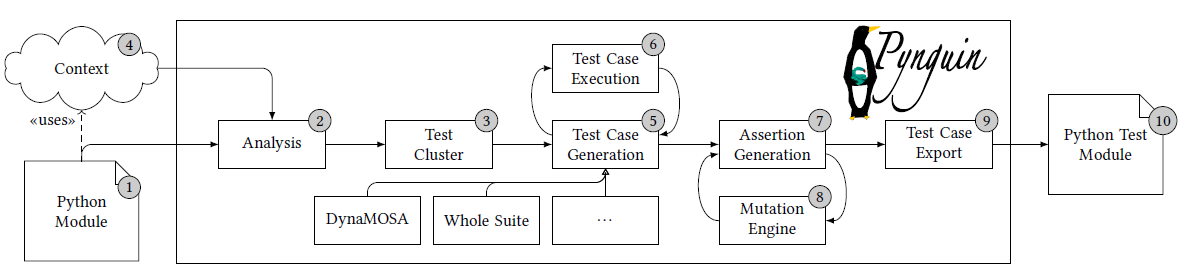
\includegraphics[width=.99\textwidth]{Figures/pynguin.png}
  \caption{Pynguin structure}\label{fig:pyn}
\end{figure}

Its structure is presented in Figure~\ref{fig:pyn} and consists of 10 autonomous steps that work in the following manner
\begin{enumerate}
  \item The unit test generation process starts with the input of a user defined python module that needs to be tested.
  \item The module is then analyzed in order to obtain primordial information, such as all the functions, classes and their respective attributes and methods, together with their respective parameters.
  \item In the Test Cluster, all the information gathered from the analysis of the module under test (MUT) and its relevant dependencies.
  \item As mentioned in the previous item, the Context step performs an interprocedural analysis of all the libraries and modules used by the actual MUT, and joins any new obtained information with the data in the Test Cluster.
  \item The Test Case Generation step, individually picks functions or methods from the Test Cluster in order to generate the internal representation, firstly by creating a statement using the function or method in question, and then generating an argument for every parameter.
  \item After a Test Case Generation is perfomed, it is executed to get the desired coverage and analyse if (a) it alreay reacher the maximum or (b) a new better Test Case should be generated.
  \item Once the stopping conditions are met, the test cases are finished with an optional assertion to check the results of the testing.
  \item Alternatively, mutations of the test cases are created using MutPY, so Pynguin can evaluate if the previously created assertion kill or not the mutants.
  If they do not, new assertions are created.
  \item In the Export step, Pynguin translates the test cases from its internal representation into test code with the format of the library PyTest.
  \item Finally, these tests are written into a final module.
  
\end{enumerate}
%Is this plagio?
At the time of its original release (25th of July 2020), Pynguin was a state of the art open source tool that has made the first step for subsequent researches about how to improve the performance and functionalities of Pynguin itself, including CodaMOSA~\cite{DBLP:conf/icse/LemieuxILS23}, PyLC~\cite{DBLP:conf/sac/SalariEAS23} and many other tools that will be breafly explained in the State of the Art section.

These recent new extensions of Pynguin and the aforementioned problem at the time of generating complex object inputs are the principal motivations of this thesis and the related and future work to it.

\iffalse{}
\begin{summary}{Structure}
\begin{itemize}
  \item test generation CHECK
  \item test generation in dynamic languages and it's difficulties CHECK
  \item pynguin and its accomplishments
\end{itemize}
\end{summary}

\fi


\chapter{Proposal}

The original Pynguin research paper~\cite{DBLP:conf/icse/LukasczykF22} stated that after the test generation of 118 Python modules, the average branch coverage over all algorithms was $66.8\%$, which leads to think that improvement is possible.
%talk about how coverage isn't everything?
The current Master's thesis proposes an addition to the original structure of Pynguin~(see~Figure~\ref{fig:pyn}), specifically to sections (5) and (2) by developing
a Graph-Based Object Synthesis approach~\cite{DBLP:conf/sigsoft/0001O00D21} and optionaly the usage of an external type inference module respectively, in order to diminish the branch coverage gap and try to generate more complex test suites.

What the Graph-Based heuristic proposed by Lin et al.~\cite{DBLP:conf/sigsoft/0001O00D21} does, is generate a object construction graph (OCG) from a previous code slicing, performed from the program dependency graph and a specific target branch as criteria.
This branch must be selected from those who have not reached their full coverage, or are ``non-trivial'', and the depth of the intraprocedural dependency should be set as a arbitrary level $t_{\text{dep}}$.
\textbf{Some explanation of the representation of code by Pynguin and its relevance to the algorithm should be explained.}
Then, this OCG is used to generate a code template that should be either translated directly into the test code representation of Pynguin or an intermediate form.
This previous idea was completely implemented in and for Java, which means that part of the work to be done is to ideate a new Python representations of the OCG.\@
The usage of a external type inference library is mentiones as optional in the hypotethical case of the branch coverage improvement not being as substantial in Pynguin as the one obtained while experimenting over EvoObj, the new instance of EvoSuit.
After implementation part is done, a study of the extension will be made through the selection of arbitrary sets of Python modules, being these either the original research paper's or a new set that ensures the explicit type of object inputs and a ratio of this kind of inputs of more than $50\%$.
The final purpose of the thesis is to obtain a Cohen's d effect size over the coverage results between Pynguin and the proposed extension either equal or bigger to the ones obtained between EvoSuite and EvoObj, being this greater than an average of $0.30$ over ¿all? possible algorithms in the different time budgets.



\begin{summary}{Objectives}
\centering\textbf{Main Objective}
\begin{itemize}
\item  Develop a Pynguin extension that generates graph-based complex object inputs.
\end{itemize}
\centering\textbf{Secondary Objectives}
\begin{itemize}
\item  Pick a set of adecuate Python modules to prove the effectiveness of the Pynguin extension
\item (Optional) Integrate Pynguin with an external type inference~library
\item Use the arbitrary set of Python modules in order to compare the public version of Pynguin with its soon to be created extension
\item Reach an increase in the effect size of the branch coverage results by a factor of $0.30$
\end{itemize}
\end{summary}

\chapter{State of the Art}

\textbf{If the state of the art papers mention different kinds of tests (unit, regression, etc), maybe its a good idea to explain them.}
\textbf{Also, some other concepts should be stated, such as acronyms for subject under test for generalization.}

\section{EvoSuite}
With respect to Unit Test Generation, EvoSuite~\cite{DBLP:conf/qsic/FraserA11} was (and still is) a state of the art test generation tool for Java, pioneer of the usage of a genetic algorithm so the branch coverage can be optimized as a whole.
The internal repesentation of EvoSuite for a test suite is a set of \textit{chromosomes} $T$ as a sequence of statements $t_i$ of length $l_i$ and either type primitive statement, constructor statement, field statement, or method statement.
During the chromosome synthesis process, all the information regarding classes, methods and variables of the SUT are gathered via the Java Bytecode and Java Reflection\footnote{https://docs.oracle.com/javase/8/docs/technotes/guides/reflection/index.html}.
These sequences can be crossovered as a random secuential combination of the two \textit{chromosomes}, or mutated with the insertion, remotion or change of single statements.
In terms of the optimization, the fitness function of a test suite $T$ is given by the equation
\[ \text{fitness}(T) = |M| - |M_T| + \sum_{b_k \in B} d(b_k, T) \]
where $M$ is the total of methods to test, $M_T$ is the number of methods that were actually executed, $b_k$ is a branch in the branch set $B$, and $d(b, T)$ is the branch distance of branch $b$ over the set $T$.
Another limitation to the suites $T$, are $N$ as the maximum number of chromosomes ($T = \{t_1, \dots , t_n\}$) and $L$ as maximum length of the chromosomes ($l_i < L$).
For the experiment phase, a single branch approach was created by the authors, in which every branch $b_t$ is seen as a single coverage goal to be met by the test cases.
Then, the comparison between the single branch method and the whole suite optimization is done with the generation of test cases for five open source projects, accumulating a total of 1308 classes from which 727 were public.
After the execution of test cases was complete and statistical tests were applied, it could be stated that the results show EvoSuite has a better branch coverage and creates smaller tests suites than the single objective method.

\section{NxtUnit}

Having EvoSuite, Randoop and Pynguin as precedents, in 2023 developers from ByteDance (technology Chinese company) presented NxtUnit~\cite{DBLP:conf/ease/WangMCGSP23}, a automatic randomized test generation tool for the programming language Go.
Similar to the state of the art tools, the structure of NxtUnit (see Figure~\ref{fig:nxt}) is composed by an initial source code as input, that is translated into Static Single Assignment form as a way to get a graph with call dependencies between functions.
After this preprocessing, NxtUnit proceeds to synthesize from the call graph a code template that will be filled with appropiate randomly generated parameters and ran during the tool's execution.
All the information for the template synthesis and posterior parameter changes will be done thanks to the information provided by Go Reflect~\footnote{https://pkg.go.dev/reflect}.
During the code running phase, NxtUnit focuses in three main tasks: mutation of the parameter inputs at runtime, assertion generation for future regression testing, and test case selection based on code coverage.
Once the tool comes to a halt, the best test cases are exported into a test suite.
In the experiment proposed by the authors, NxtUnit was executed on 500 private ByteDance repositories and 13 out of the 100 highly-rated public repositories of Go, both sets that already contain tests.
The main objective of this setup, was to review the code coverage increase while adding NxtUnit tests to the already existing ones, and it produced an avergae increase of $\%5.51$ for the public repositories and $\%17.26$ for the private ones.


\begin{figure}[bt]
  \centering
  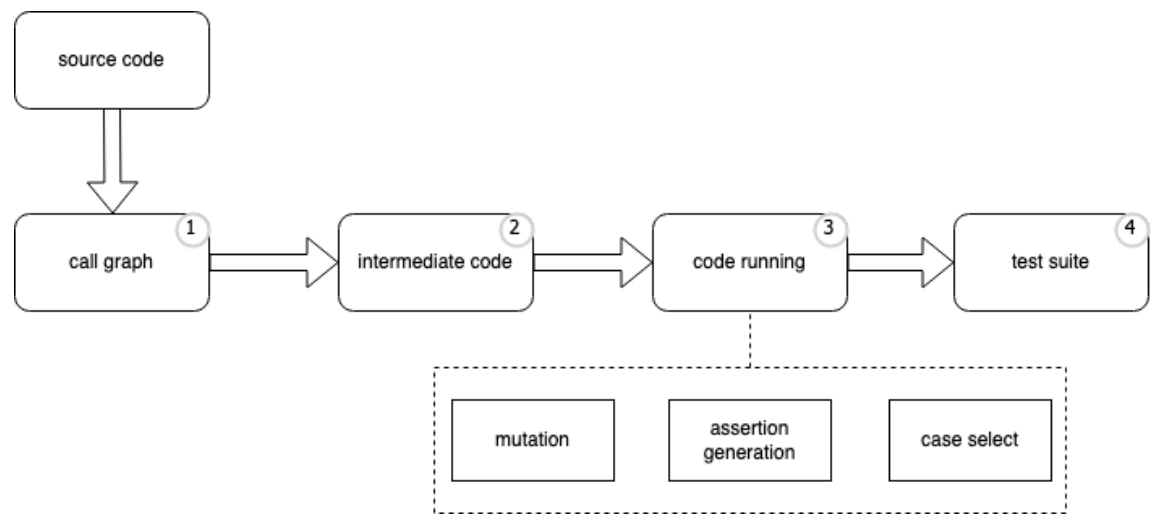
\includegraphics[width=.99\textwidth]{Figures/nxtunit.png}
  \caption{NxtUnit structure}\label{fig:nxt}
\end{figure}


\begin{itemize}
  \item state of the unit test generation in dynamic languages
  \begin{itemize}
    \item JSEFT(JS)~\cite{DBLP:conf/icst/Mirshokraie0P15}
    \item NxtUnit(GO)~\cite{DBLP:conf/ease/WangMCGSP23}
  \end{itemize}
  \item state of the unit test generation in python
  \begin{itemize}
    \item CodaMOSA~\cite{DBLP:conf/icse/LemieuxILS23}
    \item PBT-GPT~\cite{DBLP:journals/corr/abs-2307-04346}
    \item CodeT~\cite{DBLP:journals/corr/abs-2207-10397}
    \item MutAP~\cite{DBLP:journals/corr/abs-2308-16557}
    \item LExecutor~\cite{DBLP:journals/corr/abs-2302-02343}
    \item Mutester~\cite{DBLP:journals/corr/abs-2307-00404}
    \item ChatGPT~\cite{li2023nuances}
    \item PyLC~\cite{DBLP:conf/sac/SalariEAS23}
  \end{itemize}
\end{itemize}

Comments on the state of the art

\backmatter{}

\printbibliography{}

\end{document}
